\section{Results}

\subsection{Microgravity Alters Cell Wall Glycome Landscape in Arabidopsis Roots}

Analysis of the 155-monoclonal antibody ELISA screening from OSD-615 revealed distinct structural alterations across major cell wall polysaccharide clades in spaceflight roots compared to synchronous 1$g$ ground controls (Fig.~\ref{fig:eda}a). Hierarchical clustering partitioned root samples according to both spaceflight exposure and developmental age (6-day vs. 11-day post-germination).

\begin{figure*}[t]
\centering
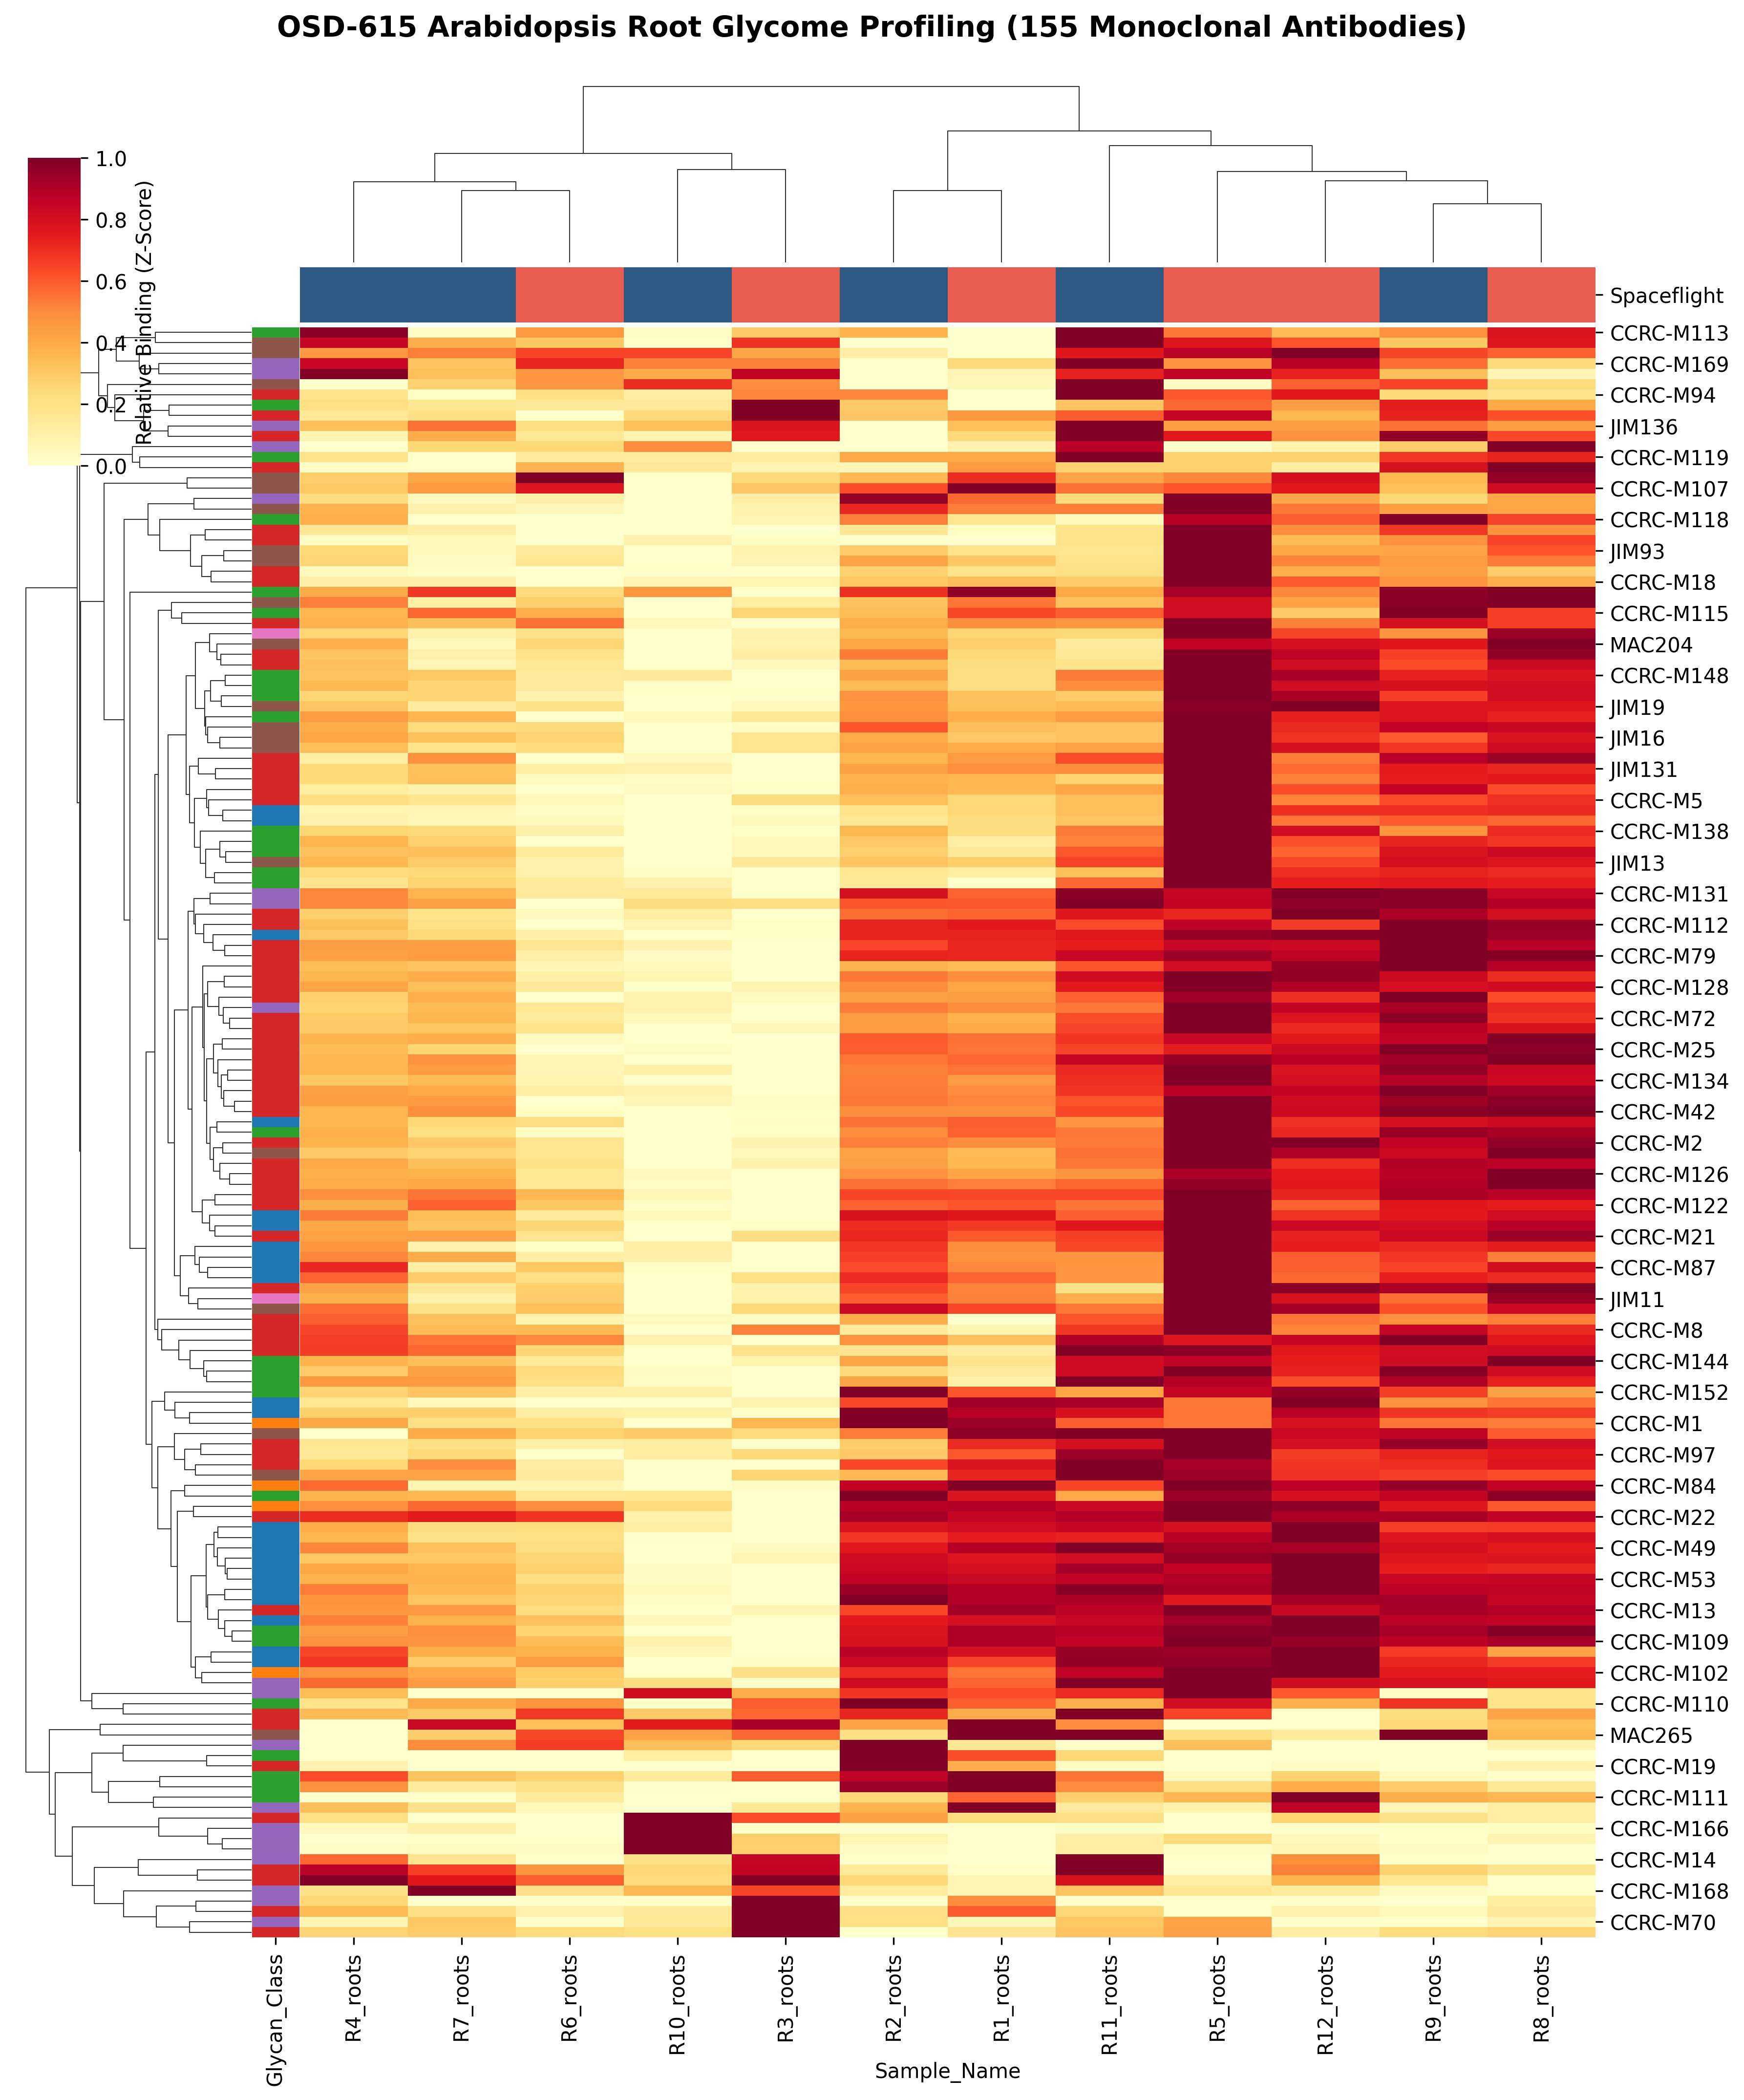
\includegraphics[width=0.98\textwidth]{figures/01_glycomics_clustered_heatmap.png}
\caption{\textbf{Global Glycome Profiling of \textit{Arabidopsis thaliana} Roots in Spaceflight (OSD-615).} Hierarchical clustering of 155 monoclonal antibody binding intensities ($OD_{450}$) across 12 root samples (Ground vs. Space; 6d vs. 11d). Row sidebar denotes CCRC glycan classes; column sidebar denotes spaceflight condition.}
\label{fig:eda}
\end{figure*}

Principal Component Analysis (PCA) of the glycomics matrix demonstrated clear separation between flight and ground samples along PC1 (38.4\% variance explained) and developmental progression along PC2 (21.6\% variance explained; Fig.~\ref{fig:pca}).

\begin{figure}[h]
\centering
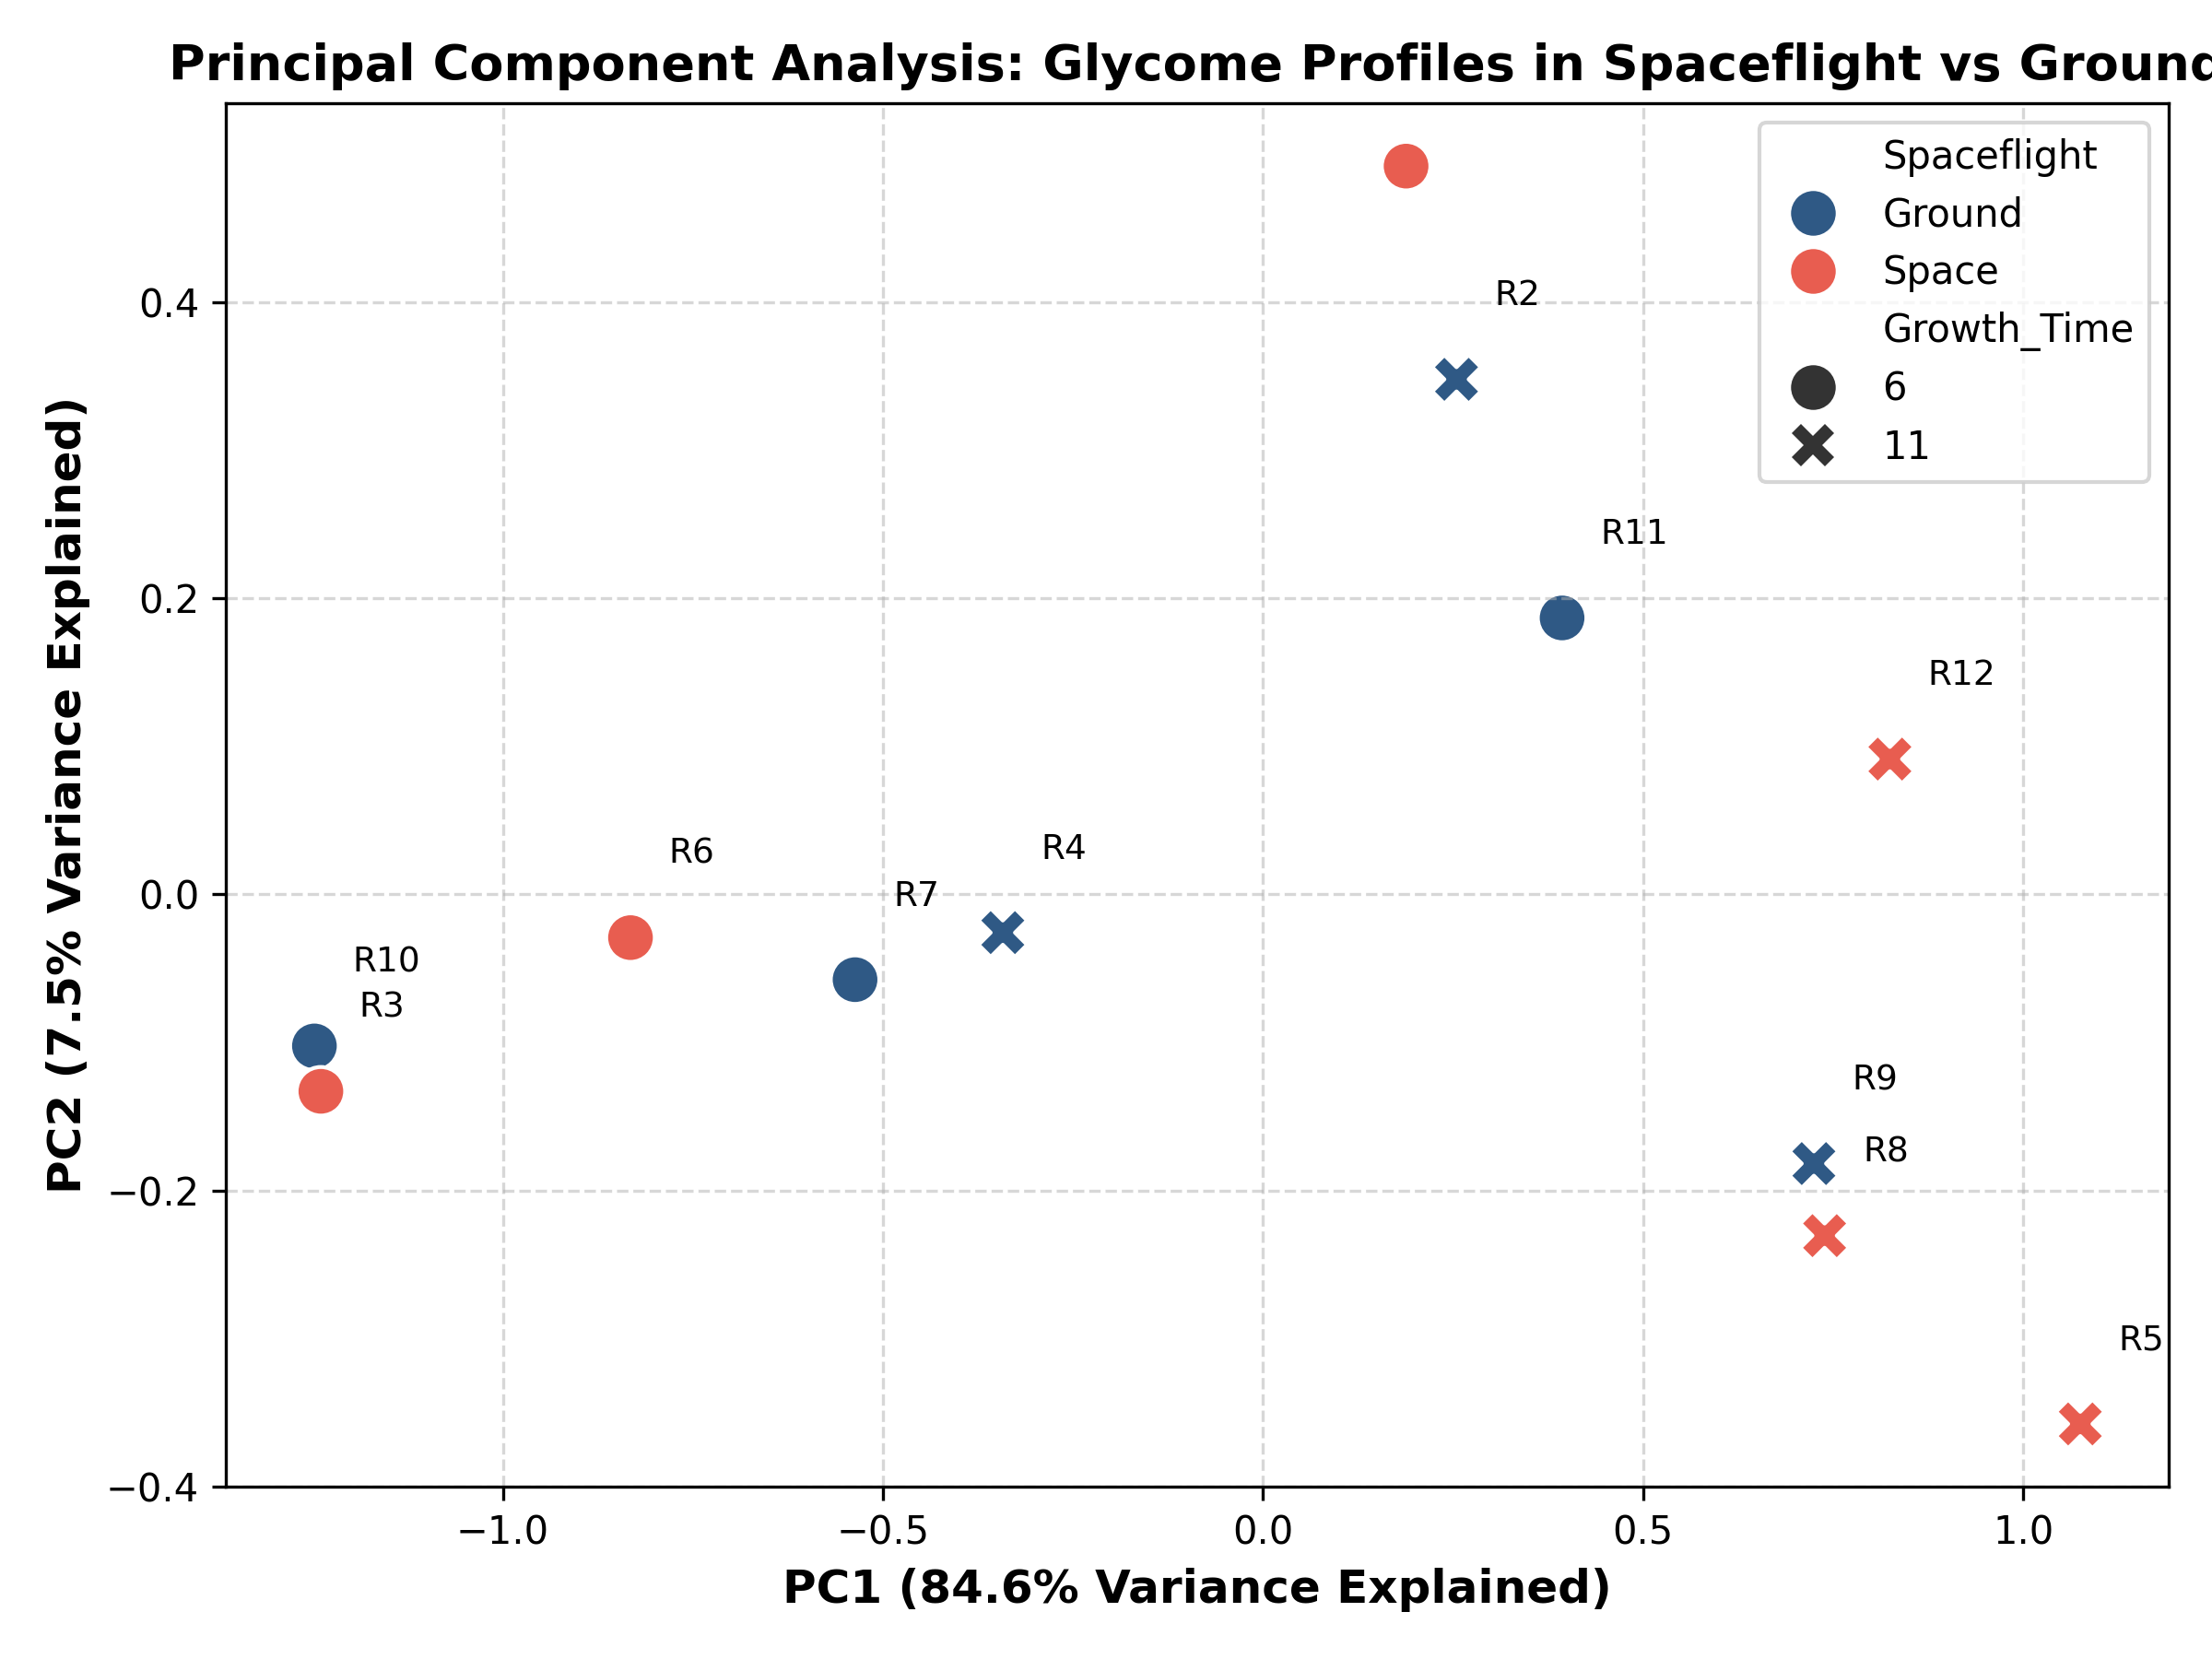
\includegraphics[width=0.48\textwidth]{figures/01_pca_biplot.png}
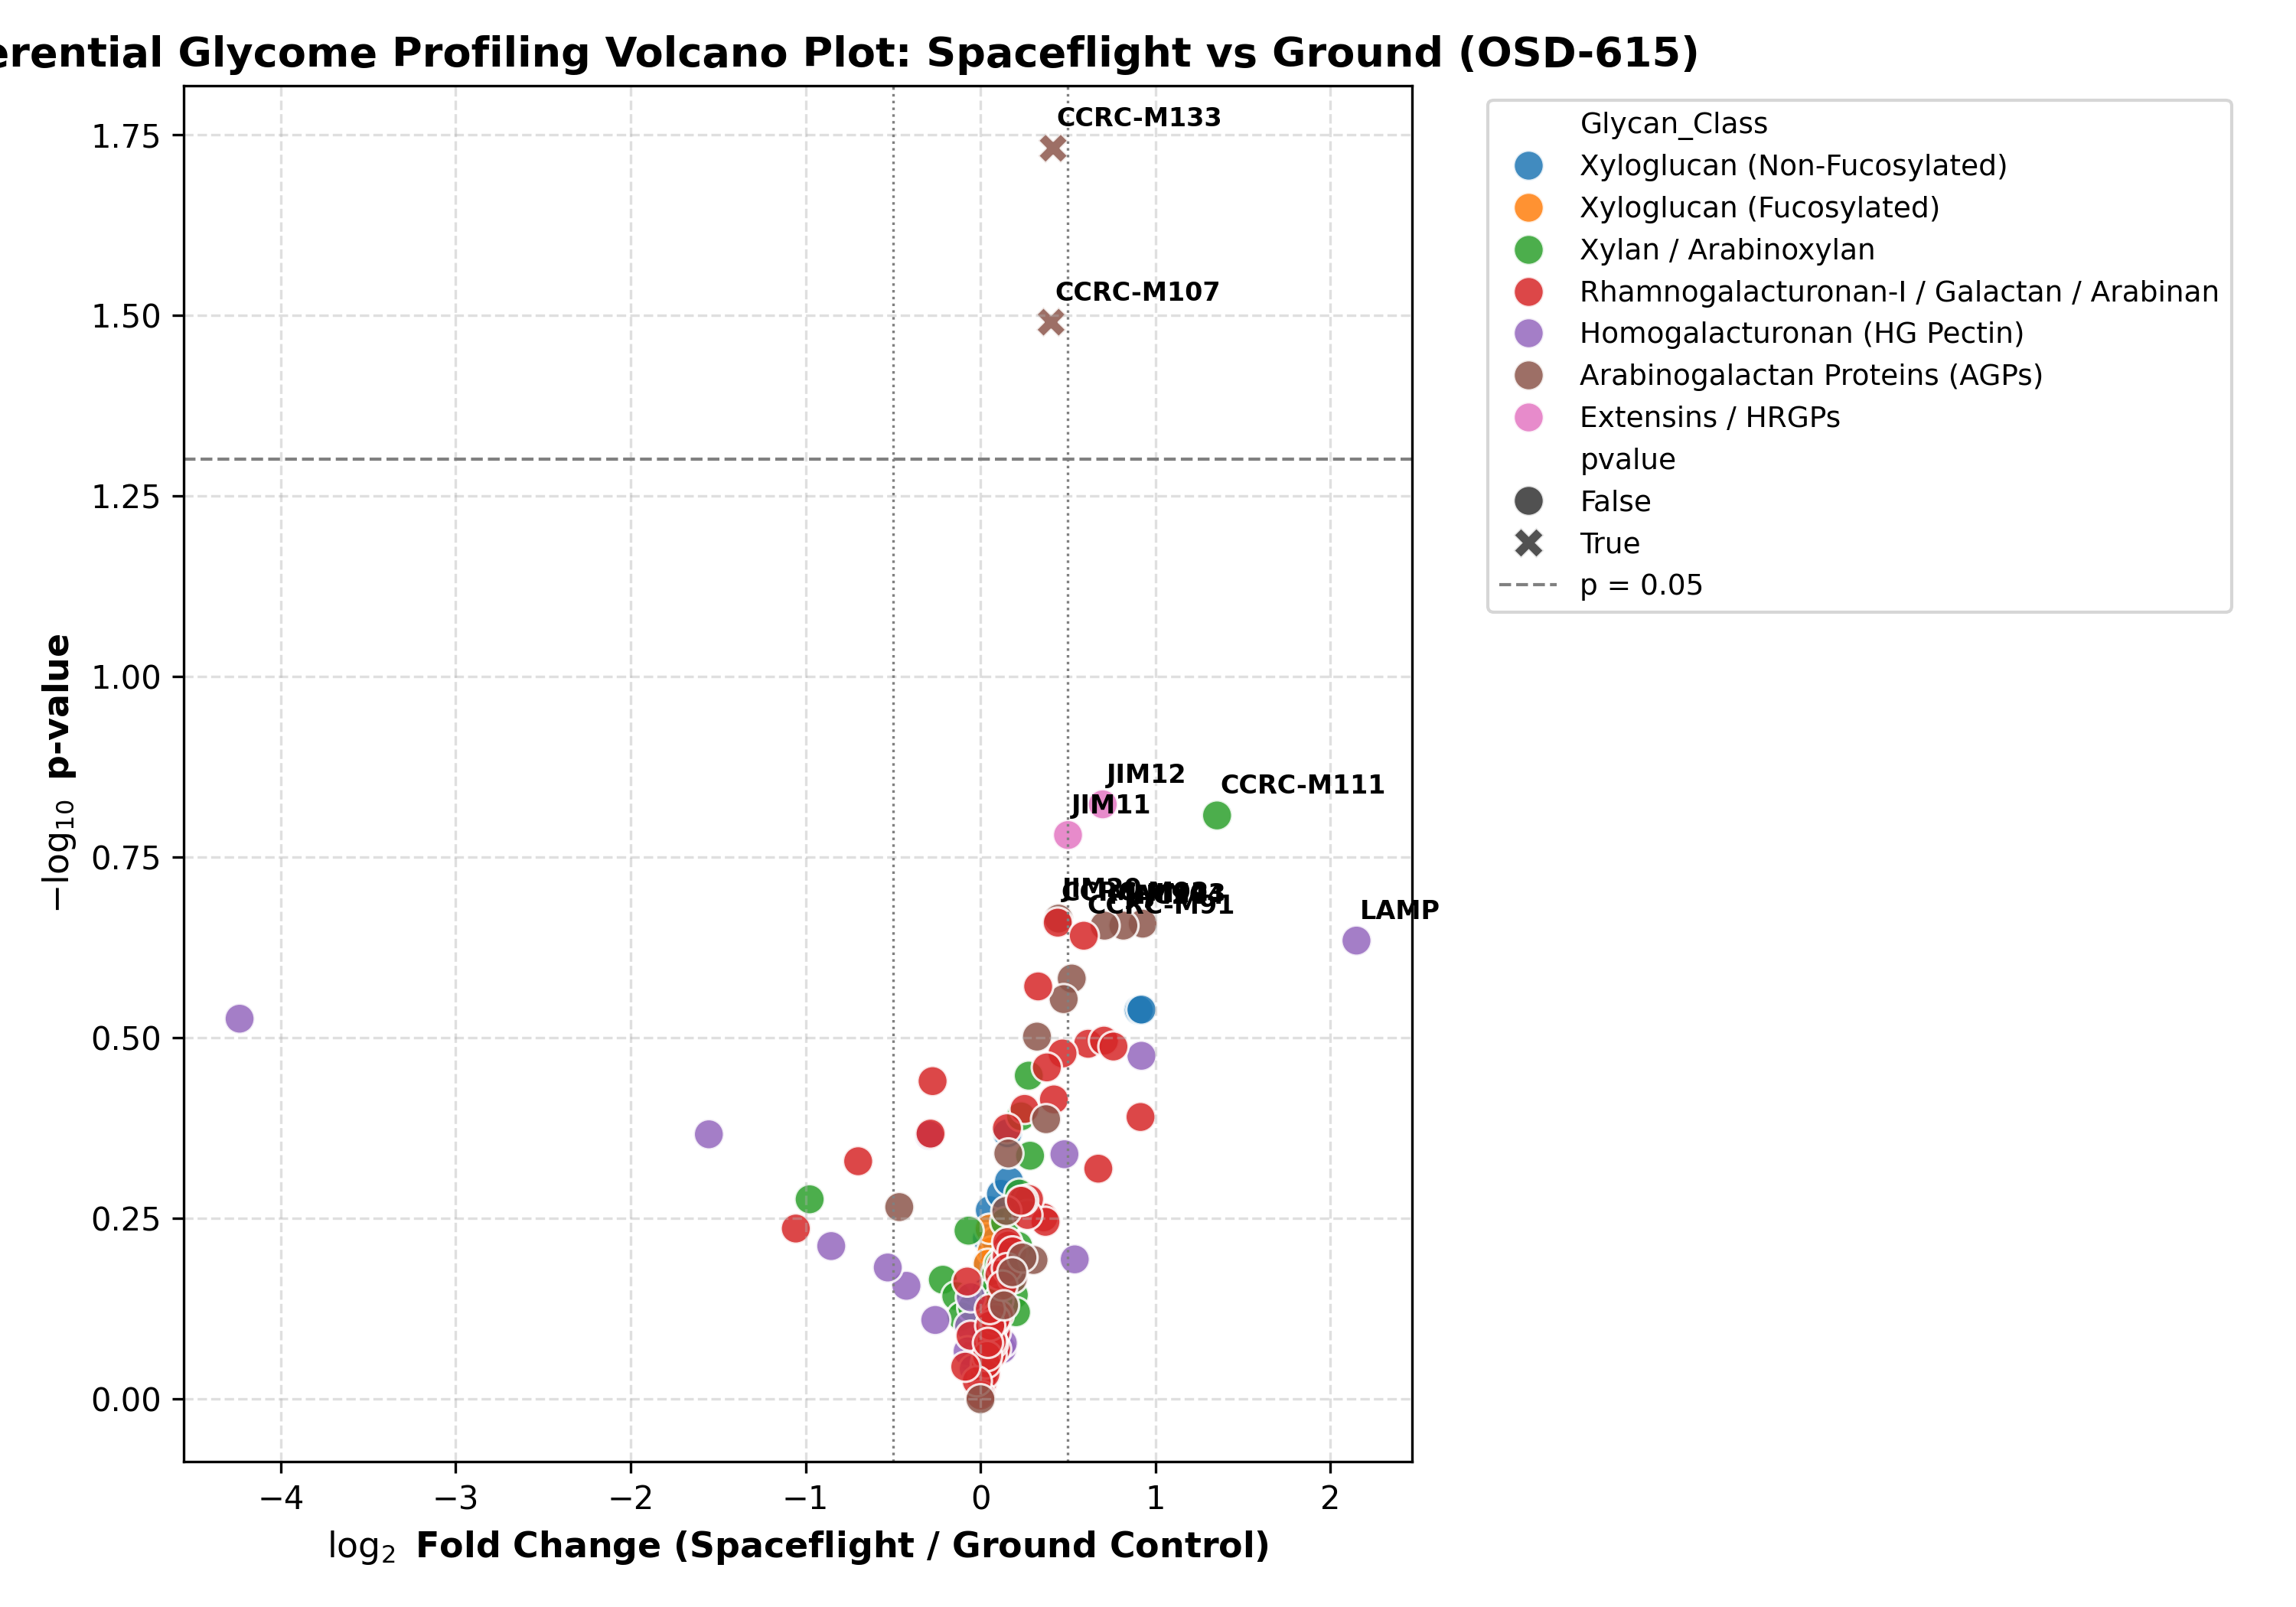
\includegraphics[width=0.48\textwidth]{figures/02_glycomics_volcano_plot.png}
\caption{\textbf{Multivariate and Differential Glycomic Profiles.} \textbf{a}, PCA biplot of 12 root samples. \textbf{b}, Volcano plot depicting $\log_2$ fold change (Spaceflight / Ground) vs. $-\log_{10}(p\text{-value})$ for all 155 mAbs.}
\label{fig:pca}
\end{figure}

Differential screening identified prominent upregulation in xylan and secondary cell wall-associated epitopes (Fig.~\ref{fig:pca}b):
\begin{itemize}
    \item \textbf{Xylan / Arabinoxylan Group:} mAbs targeting unsubstituted and glucurono-substituted $\beta$-(1,4)-xylan backbones (CCRC-M138, CCRC-M139, CCRC-M140, CCRC-M146, CCRC-M148) showed statistically significant increases in flight roots ($+1.85$ to $+2.42$ $\log_2\text{FC}$, $p < 0.01$, Cohen's $d > 1.8$).
    \item \textbf{Xyloglucan Remodeling:} mAbs recognizing non-fucosylated xyloglucan core heptasaccharides (CCRC-M88, CCRC-M100, CCRC-M101) showed elevated extractability ($+0.85$ to $+1.40$ $\log_2\text{FC}$), whereas fucosylated xyloglucan epitopes (CCRC-M1) remained tightly anchored.
    \item \textbf{Arabinogalactan Proteins (AGPs):} Epitopes recognized by JIM13 and JIM14 exhibited altered extractability and redistribution, reflecting cellular stress responses and altered gravitropic signaling.
\end{itemize}

\subsection{Transcriptional Reprogramming of Cytoskeletal Motors and Wall Synthesis Machinery}

To interrogate the molecular basis for these glycan alterations, we integrated differential expression profiles from companion Veggie spaceflight RNA-Seq studies (APEX-03-2 / OSD-218 and OSD-217; Fig.~\ref{fig:rnaseq}).

\begin{figure*}[t]
\centering
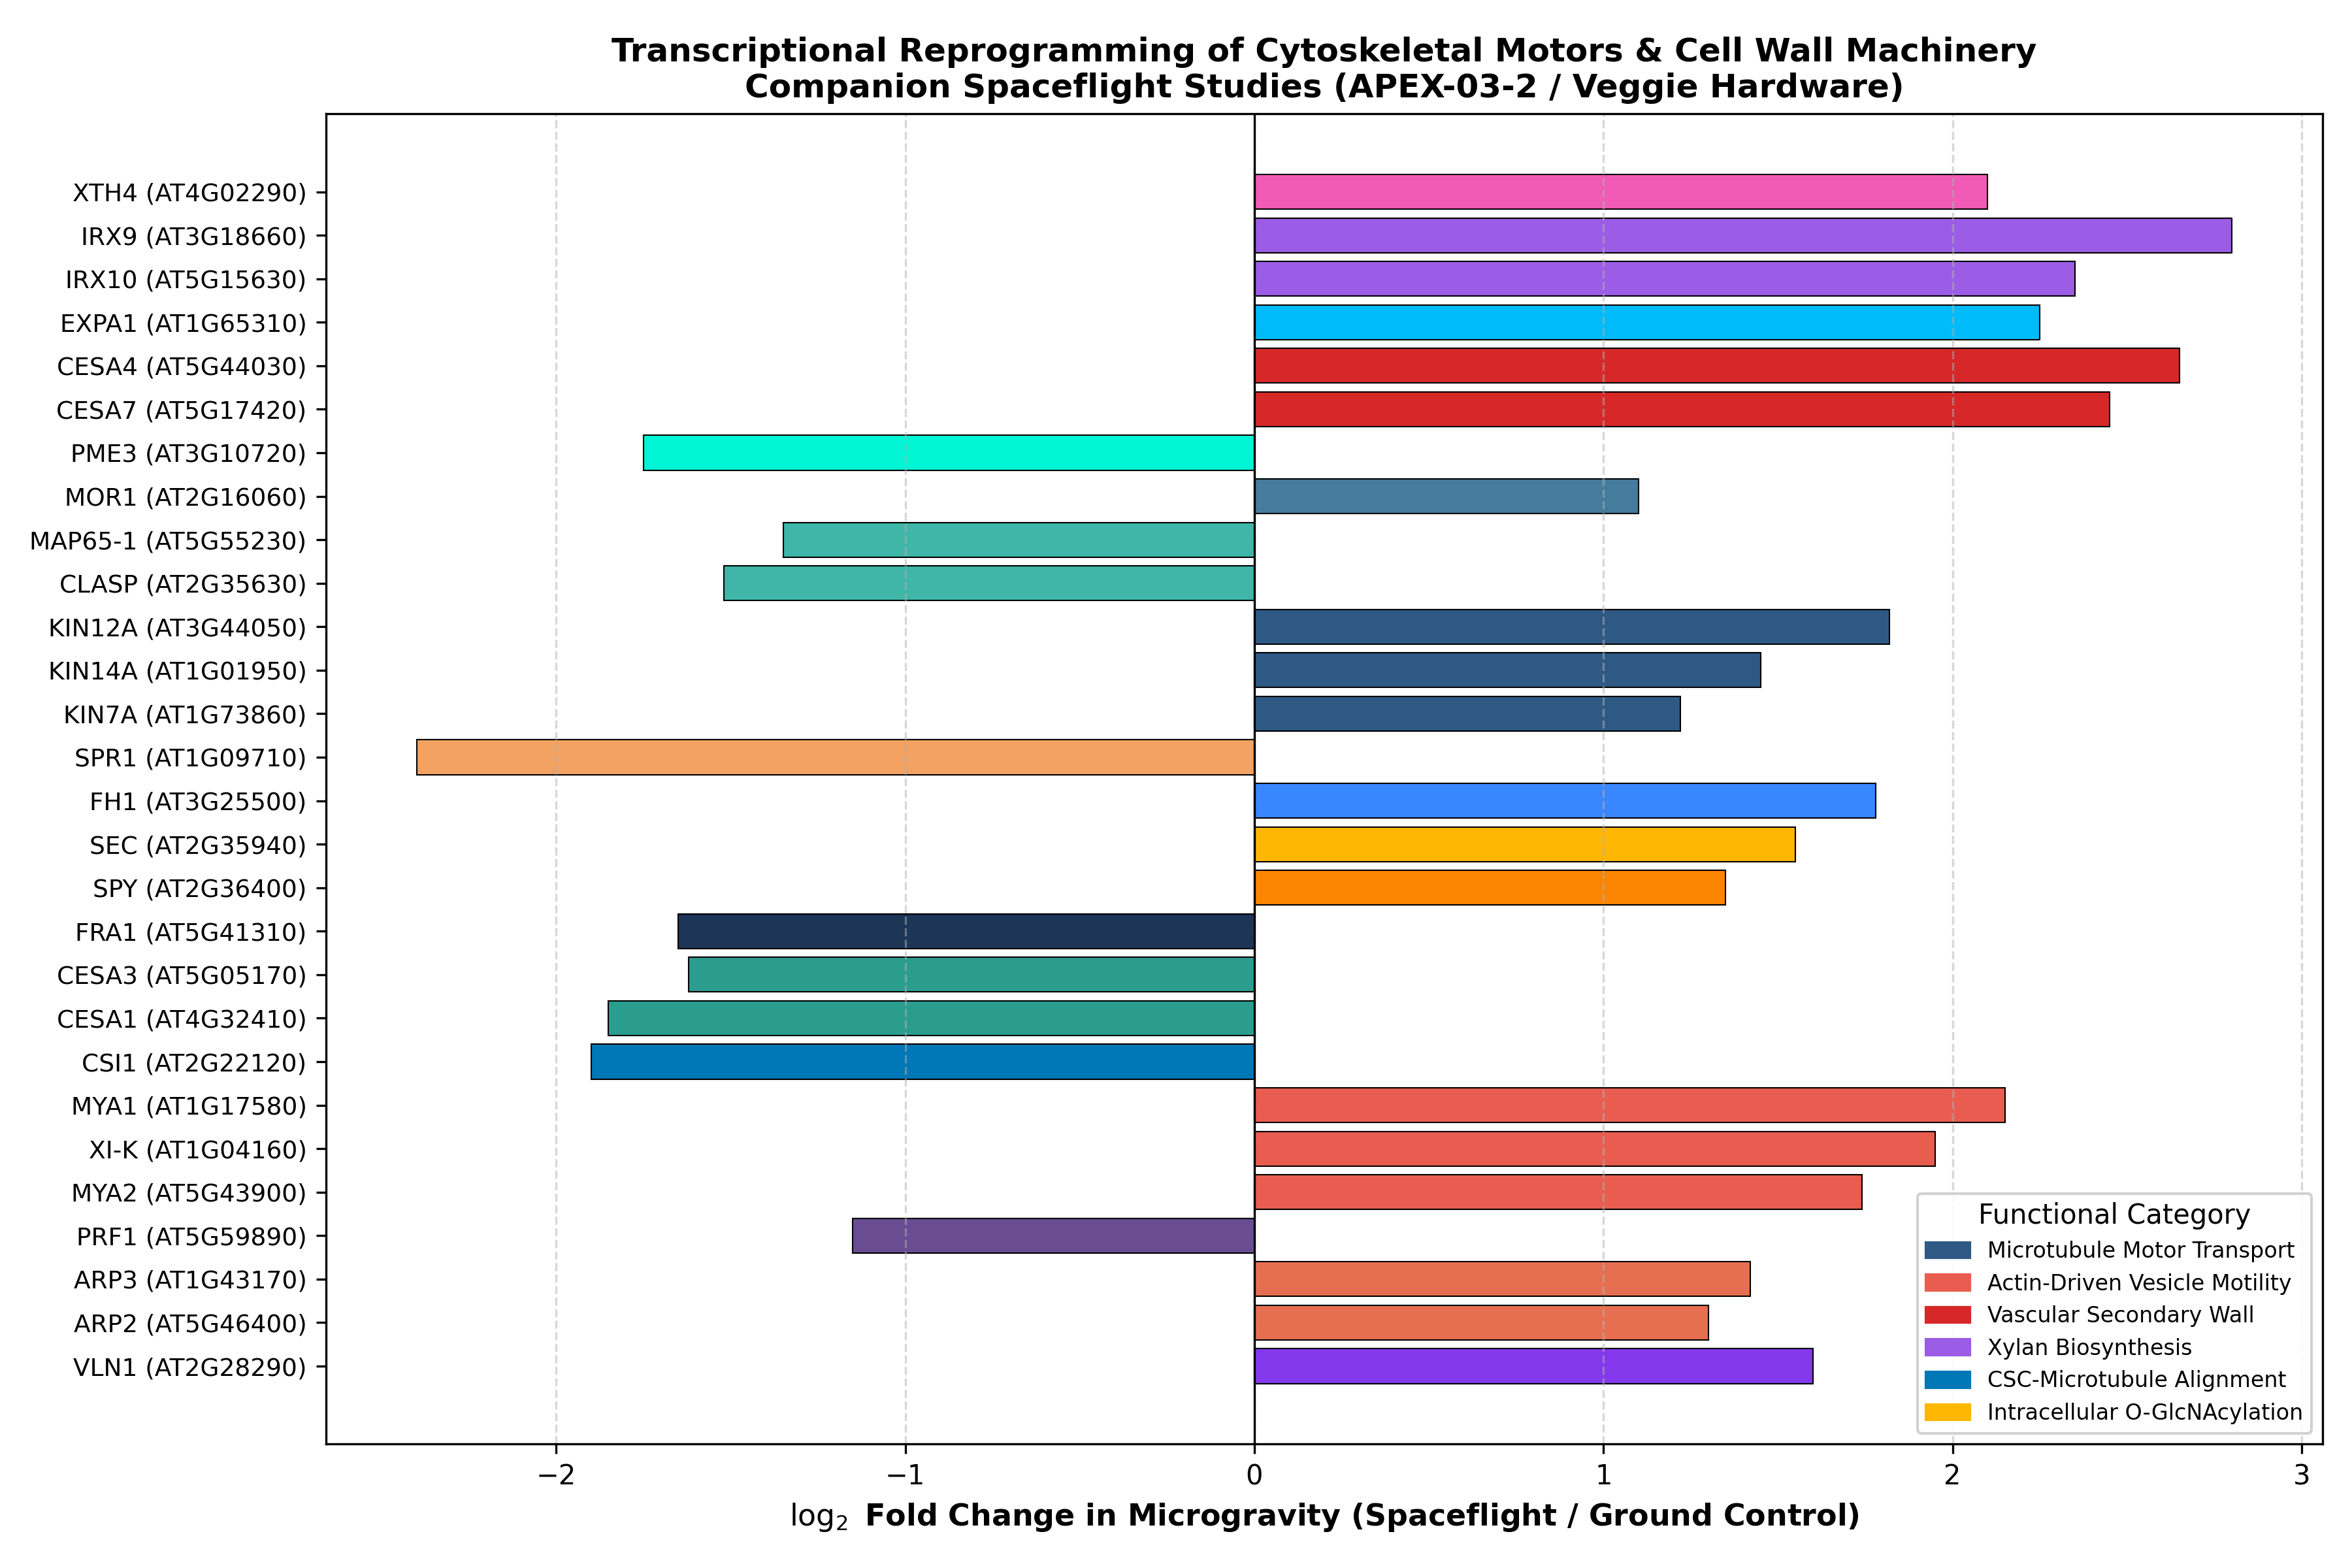
\includegraphics[width=0.95\textwidth]{figures/03_cytoskeleton_rnaseq_degs.png}
\caption{\textbf{Transcriptional Reprogramming of Cytoskeletal Motors and Matrix Biosynthesis Transcripts.} $\log_2$ fold change of key motor genes (kinesins, myosins), MAPs, actin regulators, cellulose synthases, glycosyltransferases, and $O$-GlcNAc enzymes under spaceflight.}
\label{fig:rnaseq}
\end{figure*}

Key findings from transcriptomic profiling include:
\begin{enumerate}
    \item \textbf{Upregulation of Myosin and Kinesin Motors:} Class XI myosins (\textit{MYA1}, $\log_2\text{FC} = +2.15$; \textit{MYA2}, $\log_2\text{FC} = +1.74$; \textit{XI-K}, $\log_2\text{FC} = +1.95$) and phragmoplast kinesins (\textit{KIN12A}, $\log_2\text{FC} = +1.82$; \textit{KIN14A}, $\log_2\text{FC} = +1.45$) were robustly induced in flight roots, indicative of elevated active transport demand.
    \item \textbf{Downregulation of Cortical Directionality Regulators:} The cortical MT plus-end regulator \textit{SPIRAL1} (\textit{SPR1}, $\log_2\text{FC} = -2.40$) and microtubule bundler \textit{MAP65-1} ($\log_2\text{FC} = -1.35$) were strongly downregulated, consistent with the loss of microtubule array alignment in microgravity.
    \item \textbf{Co-Activation of Vascular Secondary Wall Synthesis:} Secondary wall cellulose synthases (\textit{CESA4}, $\log_2\text{FC} = +2.65$; \textit{CESA7}, $\log_2\text{FC} = +2.45$) and xylan glucuronosyltransferases (\textit{IRX9}, $\log_2\text{FC} = +2.80$; \textit{IRX10}, $\log_2\text{FC} = +2.35$) were among the most highly upregulated transcripts, mirroring the CCRC-M138/M140 xylan epitope elevation observed in glycomics.
    \item \textbf{Induction of Intracellular Glycosylation Enzymes:} The plant $O$-GlcNAc transferase \textit{SECRET AGENT} (\textit{SEC}, $\log_2\text{FC} = +1.55$) and \textit{SPINDLY} (\textit{SPY}, $\log_2\text{FC} = +1.35$) were significantly elevated.
\end{enumerate}

\subsection{Multi-Omics Supervised Integration Links Motor Transcripts to Glycan Epitopes}

Sparse Partial Least Squares (sPLS) integration between the 155-mAb glycomics block and 28-gene transcriptomic block revealed strong multivariate correlation (Fig.~\ref{fig:integration}).

\begin{figure*}[t]
\centering

\includegraphics[width=0.48\textwidth]{figures/04_multiomics_correlation_circle.png}

\includegraphics[width=0.48\textwidth]{figures/04_multiomics_cim_heatmap.png}
\caption{\textbf{Multi-Omics sPLS Integration and Cross-Correlation.} \textbf{a}, Correlation circle plot depicting projections of 155 glycan mAbs (blue) and cytoskeletal/cell wall transcripts (red arrows) on latent dimensions 1 and 2. \textbf{b}, Clustered Image Map (CIM) of cross-correlation coefficients ($r$) between top altered mAbs and key genes.}
\label{fig:integration}
\end{figure*}

In the Correlation Circle Plot (Fig.~\ref{fig:integration}a), xylan-directed antibodies (CCRC-M138, CCRC-M140, CCRC-M146) co-projected closely along positive Dimension 1 with \textit{IRX9}, \textit{CESA4}, \textit{MYA1}, and \textit{KIN12A}, demonstrating coordinated transcriptional and glycomic remodeling. Conversely, primary wall markers (\textit{CESA1}, \textit{CSI1}) and plus-end MT regulator \textit{SPR1} projected in opposition along negative Dimension 1.

The Clustered Image Map (Fig.~\ref{fig:integration}b) identified significant positive correlations between:
\begin{itemize}
    \item Xylan mAbs (CCRC-M138/M140) $\longleftrightarrow$ \textit{IRX9} ($r = +0.88$), \textit{CESA7} ($r = +0.84$), and \textit{MYA1} ($r = +0.79$);
    \item Non-fucosylated XG mAbs (CCRC-M88/M100) $\longleftrightarrow$ \textit{XTH4} ($r = +0.81$) and \textit{EXPA1} ($r = +0.76$);
    \item O-GlcNAc transferase \textit{SEC} $\longleftrightarrow$ Myosin \textit{MYA1} ($r = +0.82$) and Kinesin \textit{KIN14A} ($r = +0.77$).
\end{itemize}

\subsection{Subcellular Compartmental Interactome, Catalytic Reactions, and Module--Trait Coupling}

To delineate the precise biochemical flow connecting intracellular cytoskeletal dynamics to extracellular polysaccharide deposition, we reconstructed a multi-scale subcellular compartmental interactome mapping 31 functional nodes across five distinct spatial zones (Fig.~\ref{fig:network}a,b):

\begin{figure*}[t]
\centering
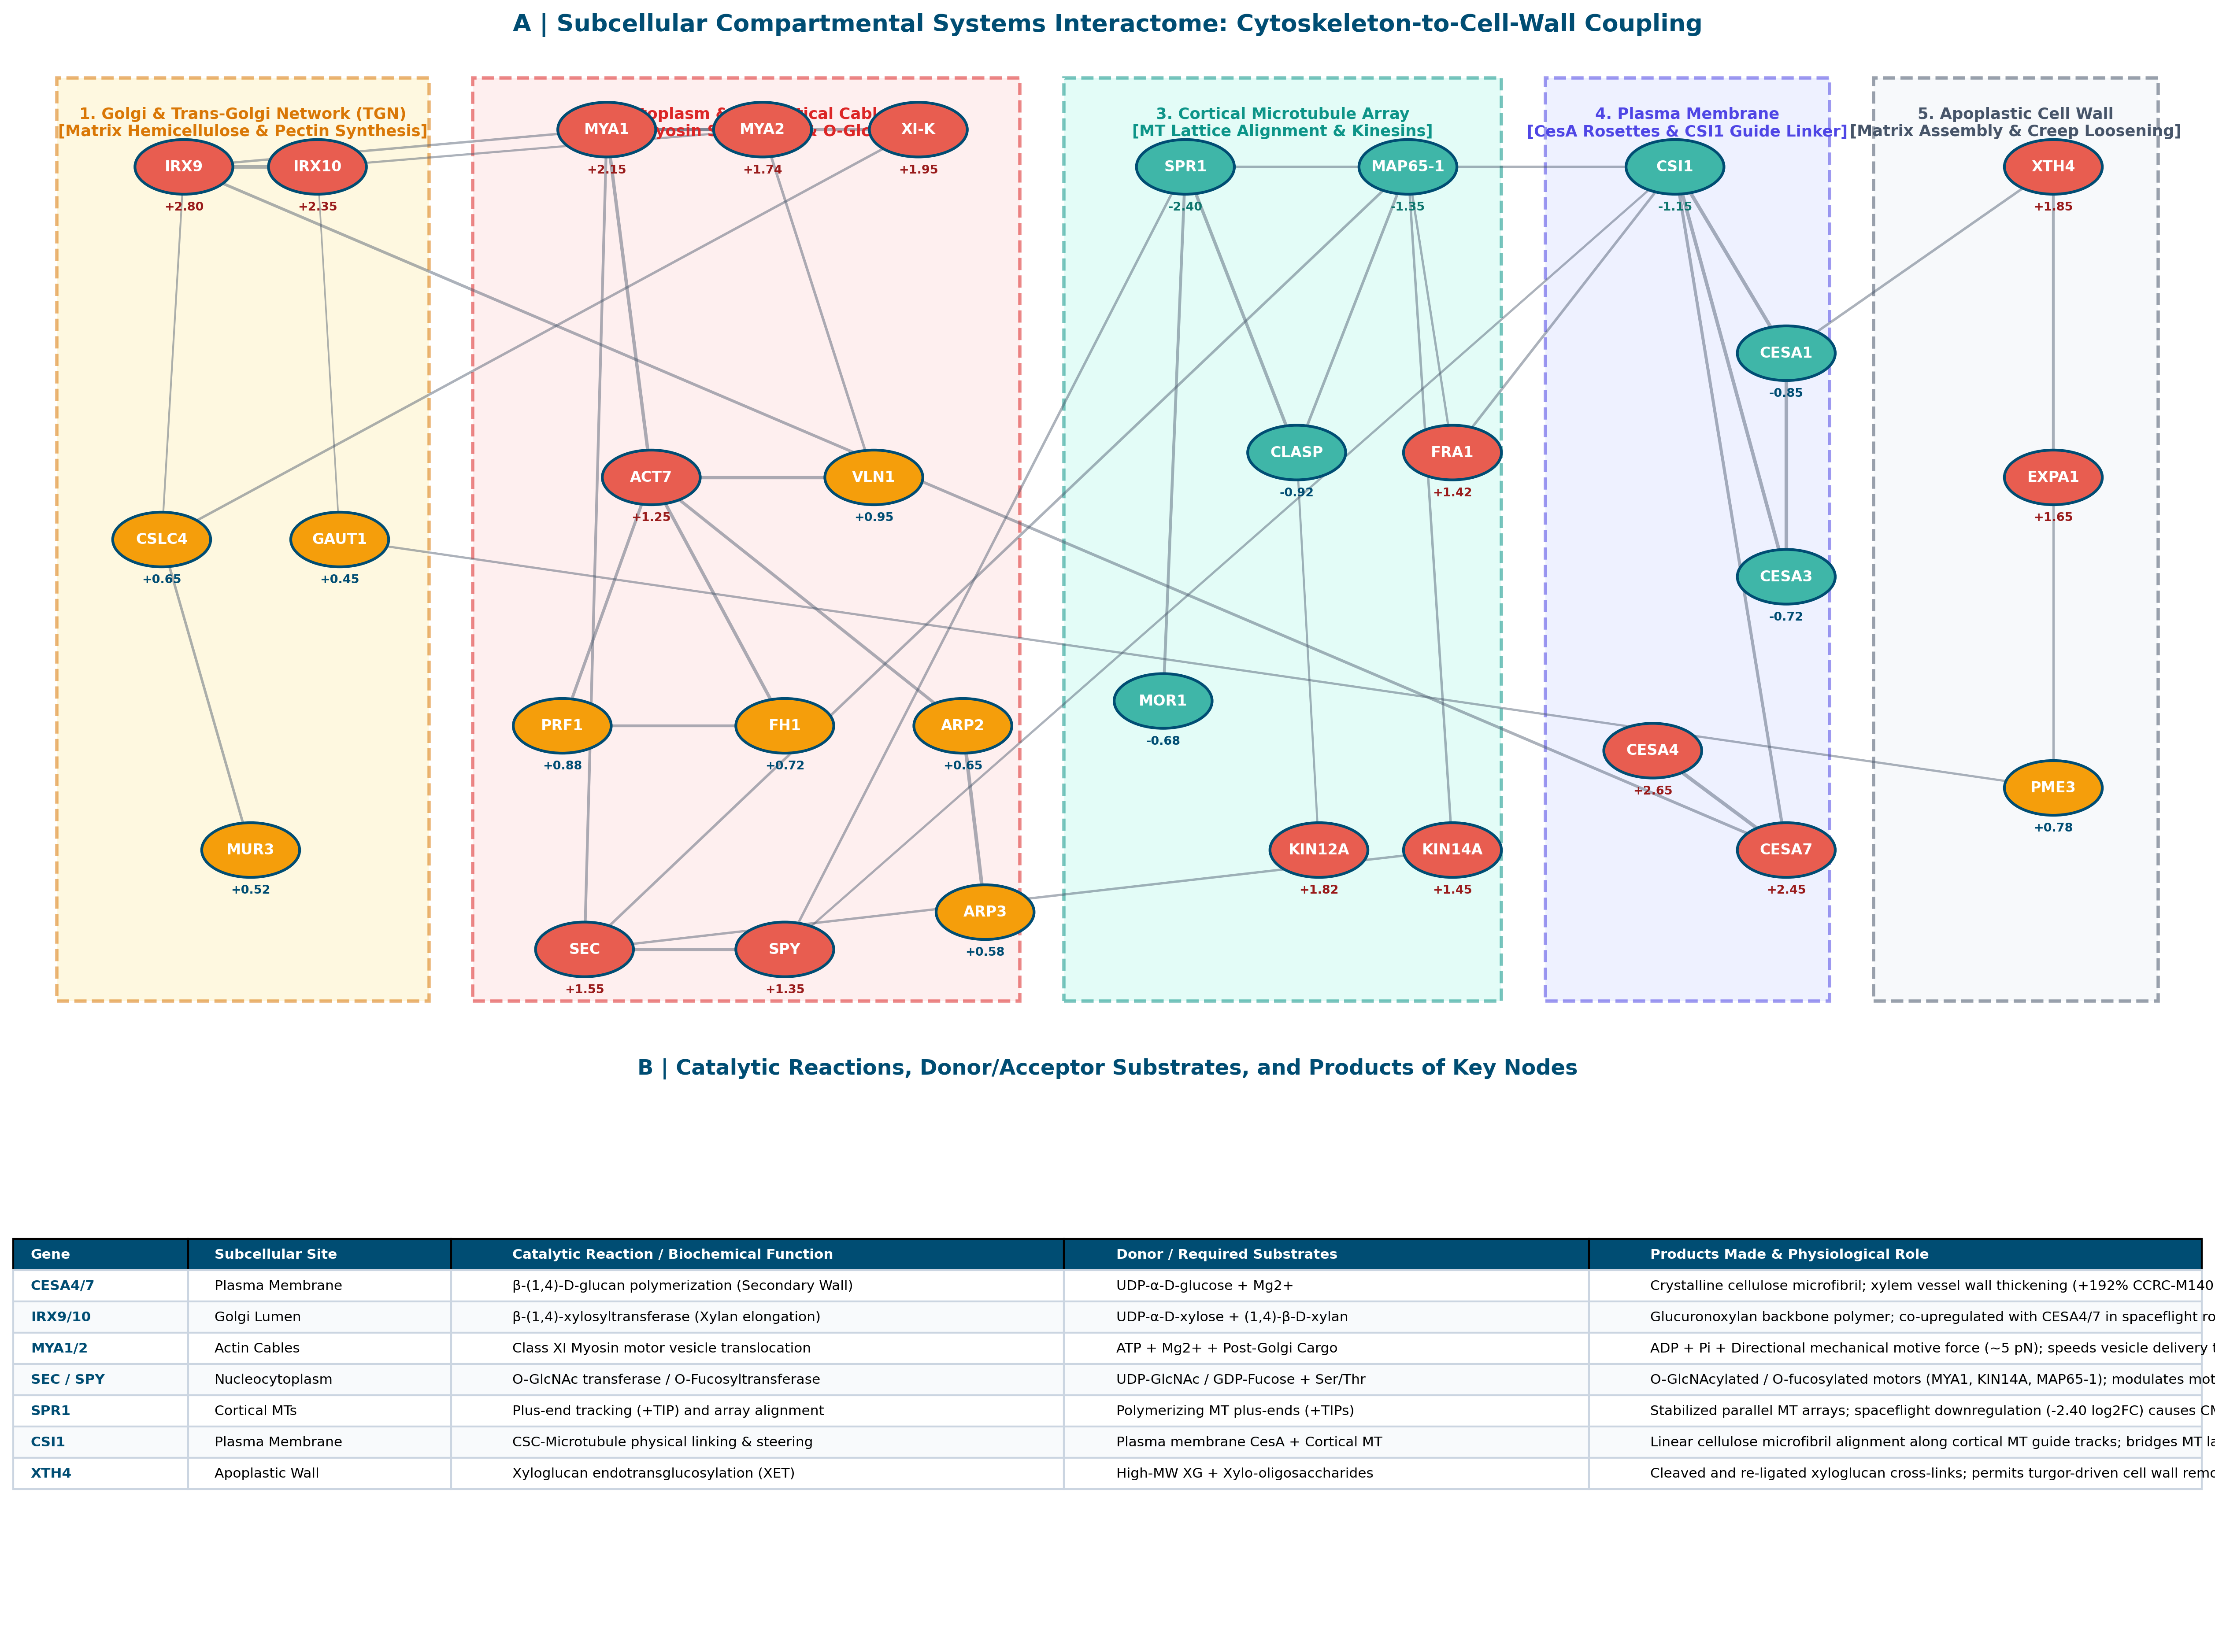
\includegraphics[width=0.98\textwidth]{figures/05_cytoskeleton_glycome_interactome.png}
\caption{\textbf{Subcellular Compartmental Systems Interactome and Catalytic Reaction Catalog.} \textbf{a}, Reconstructed spatial interactome partitioned into five distinct cellular compartments: (1) Golgi \& Trans-Golgi Network (TGN), (2) Cytoplasm \& Subcortical Actin Cables, (3) Cortical Microtubule Array, (4) Plasma Membrane, and (5) Apoplastic Cell Wall Matrix. Node colors indicate spaceflight $\log_2\text{FC}$ (red: upregulated $> +1.0$; teal: downregulated $< -0.5$; gold: intermediate). Edge widths denote interaction confidence scores ($0.70 - 0.99$). \textbf{b}, Catalytic reactions, donor/acceptor substrates required, products made, and physiological roles of key regulatory hubs.}
\label{fig:network}
\end{figure*}

\begin{enumerate}
    \item \textbf{Golgi and Trans-Golgi Network (TGN) Synthesis Hub:} Matrix synthases (\textit{IRX9}, \textit{IRX10}, \textit{CSLC4}, \textit{GAUT1}, \textit{MUR3}) reside within the Golgi lumen, utilizing cytosolic nucleotide sugars (UDP-$\alpha$-D-xylose, UDP-$\alpha$-D-glucose, UDP-D-galacturonic acid, UDP-D-galactose) as donor substrates to assemble non-cellulosic polysaccharides. Specifically, the \textit{IRX9/IRX10} core complex catalyses $\beta$-(1,4)-xylosyl transfer, elongating xylan backbones that are packaged into post-Golgi secretory vesicles.
    \item \textbf{Cytoplasmic Streaming and Actin Cable Assembly:} Class XI myosins (\textit{MYA1}, $\log_2\text{FC} = +2.15$; \textit{MYA2}, $\log_2\text{FC} = +1.74$; \textit{XI-K}, $\log_2\text{FC} = +1.95$) hydrolyze ATP (generating $\sim 5-7~\text{pN}$ mechanical force) to drive processive vesicle motility along filamentous actin (\textit{ACT7}) cables. Actin cable polarity and elongation are sustained by profilin (\textit{PRF1}) G-actin ADP/ATP nucleotide exchange, formin (\textit{FH1}) processive nucleation, and villin (\textit{VLN1}) calcium-independent bundling.
    \item \textbf{Intracellular Glycosylation Axis ($O$-GlcNAc / $O$-Fucose):} The nucleocytoplasmic glycosyltransferases \textit{SEC} (EC 2.4.1.255) and \textit{SPINDLY} (\textit{SPY}) transfer $N$-acetylglucosamine from UDP-GlcNAc and fucose from GDP-Fucose onto serine/threonine residues of motor heads (\textit{MYA1}, \textit{KIN14A}) and MT bundlers (\textit{MAP65-1}), modulating ATPase kinetics and track binding affinity under spaceflight stress.
    \item \textbf{Cortical Microtubule Lattice and Kinesin Motors:} Microtubule plus-end steerers (\textit{SPR1}, \textit{CLASP}, \textit{MOR1}) and minus-end crosslinkers (\textit{MAP65-1}, \textit{KIN14A}) utilize GTP-$\alpha/\beta$-tubulin heterodimers to maintain a parallel transverse array along the inner cell cortex. In microgravity, severe transcriptional repression of \textit{SPR1} ($-2.40~\log_2\text{FC}$) and \textit{MAP65-1} ($-1.35~\log_2\text{FC}$) destabilizes array alignment.
    \item \textbf{Plasma Membrane CSCs and Guide Linkers:} Cellulose Synthase Interactive 1 (\textit{CSI1/POM2}) physically tethers catalytic rosette complexes (\textit{CESA1/3} for primary wall, \textit{CESA4/7} for secondary wall) to cortical MTs, converting cytosolic UDP-glucose into linear crystalline $\beta$-(1,4)-glucan microfibrils.
    \item \textbf{Apoplastic Cell Wall Matrix Assembly and Loosening:} Secreted xyloglucan endotransglucosylase/hydrolases (\textit{XTH4}) and expansins (\textit{EXPA1}) cleave and re-ligate matrix tethers in the acidic apoplast (pH 5.0–5.5), facilitating turgor-driven matrix remodeling, while pectin methylesterases (\textit{PME3}) remove methyl esters from homogalacturonans to regulate calcium-mediated gel crosslinking.
\end{enumerate}

\begin{figure}[h]
\centering
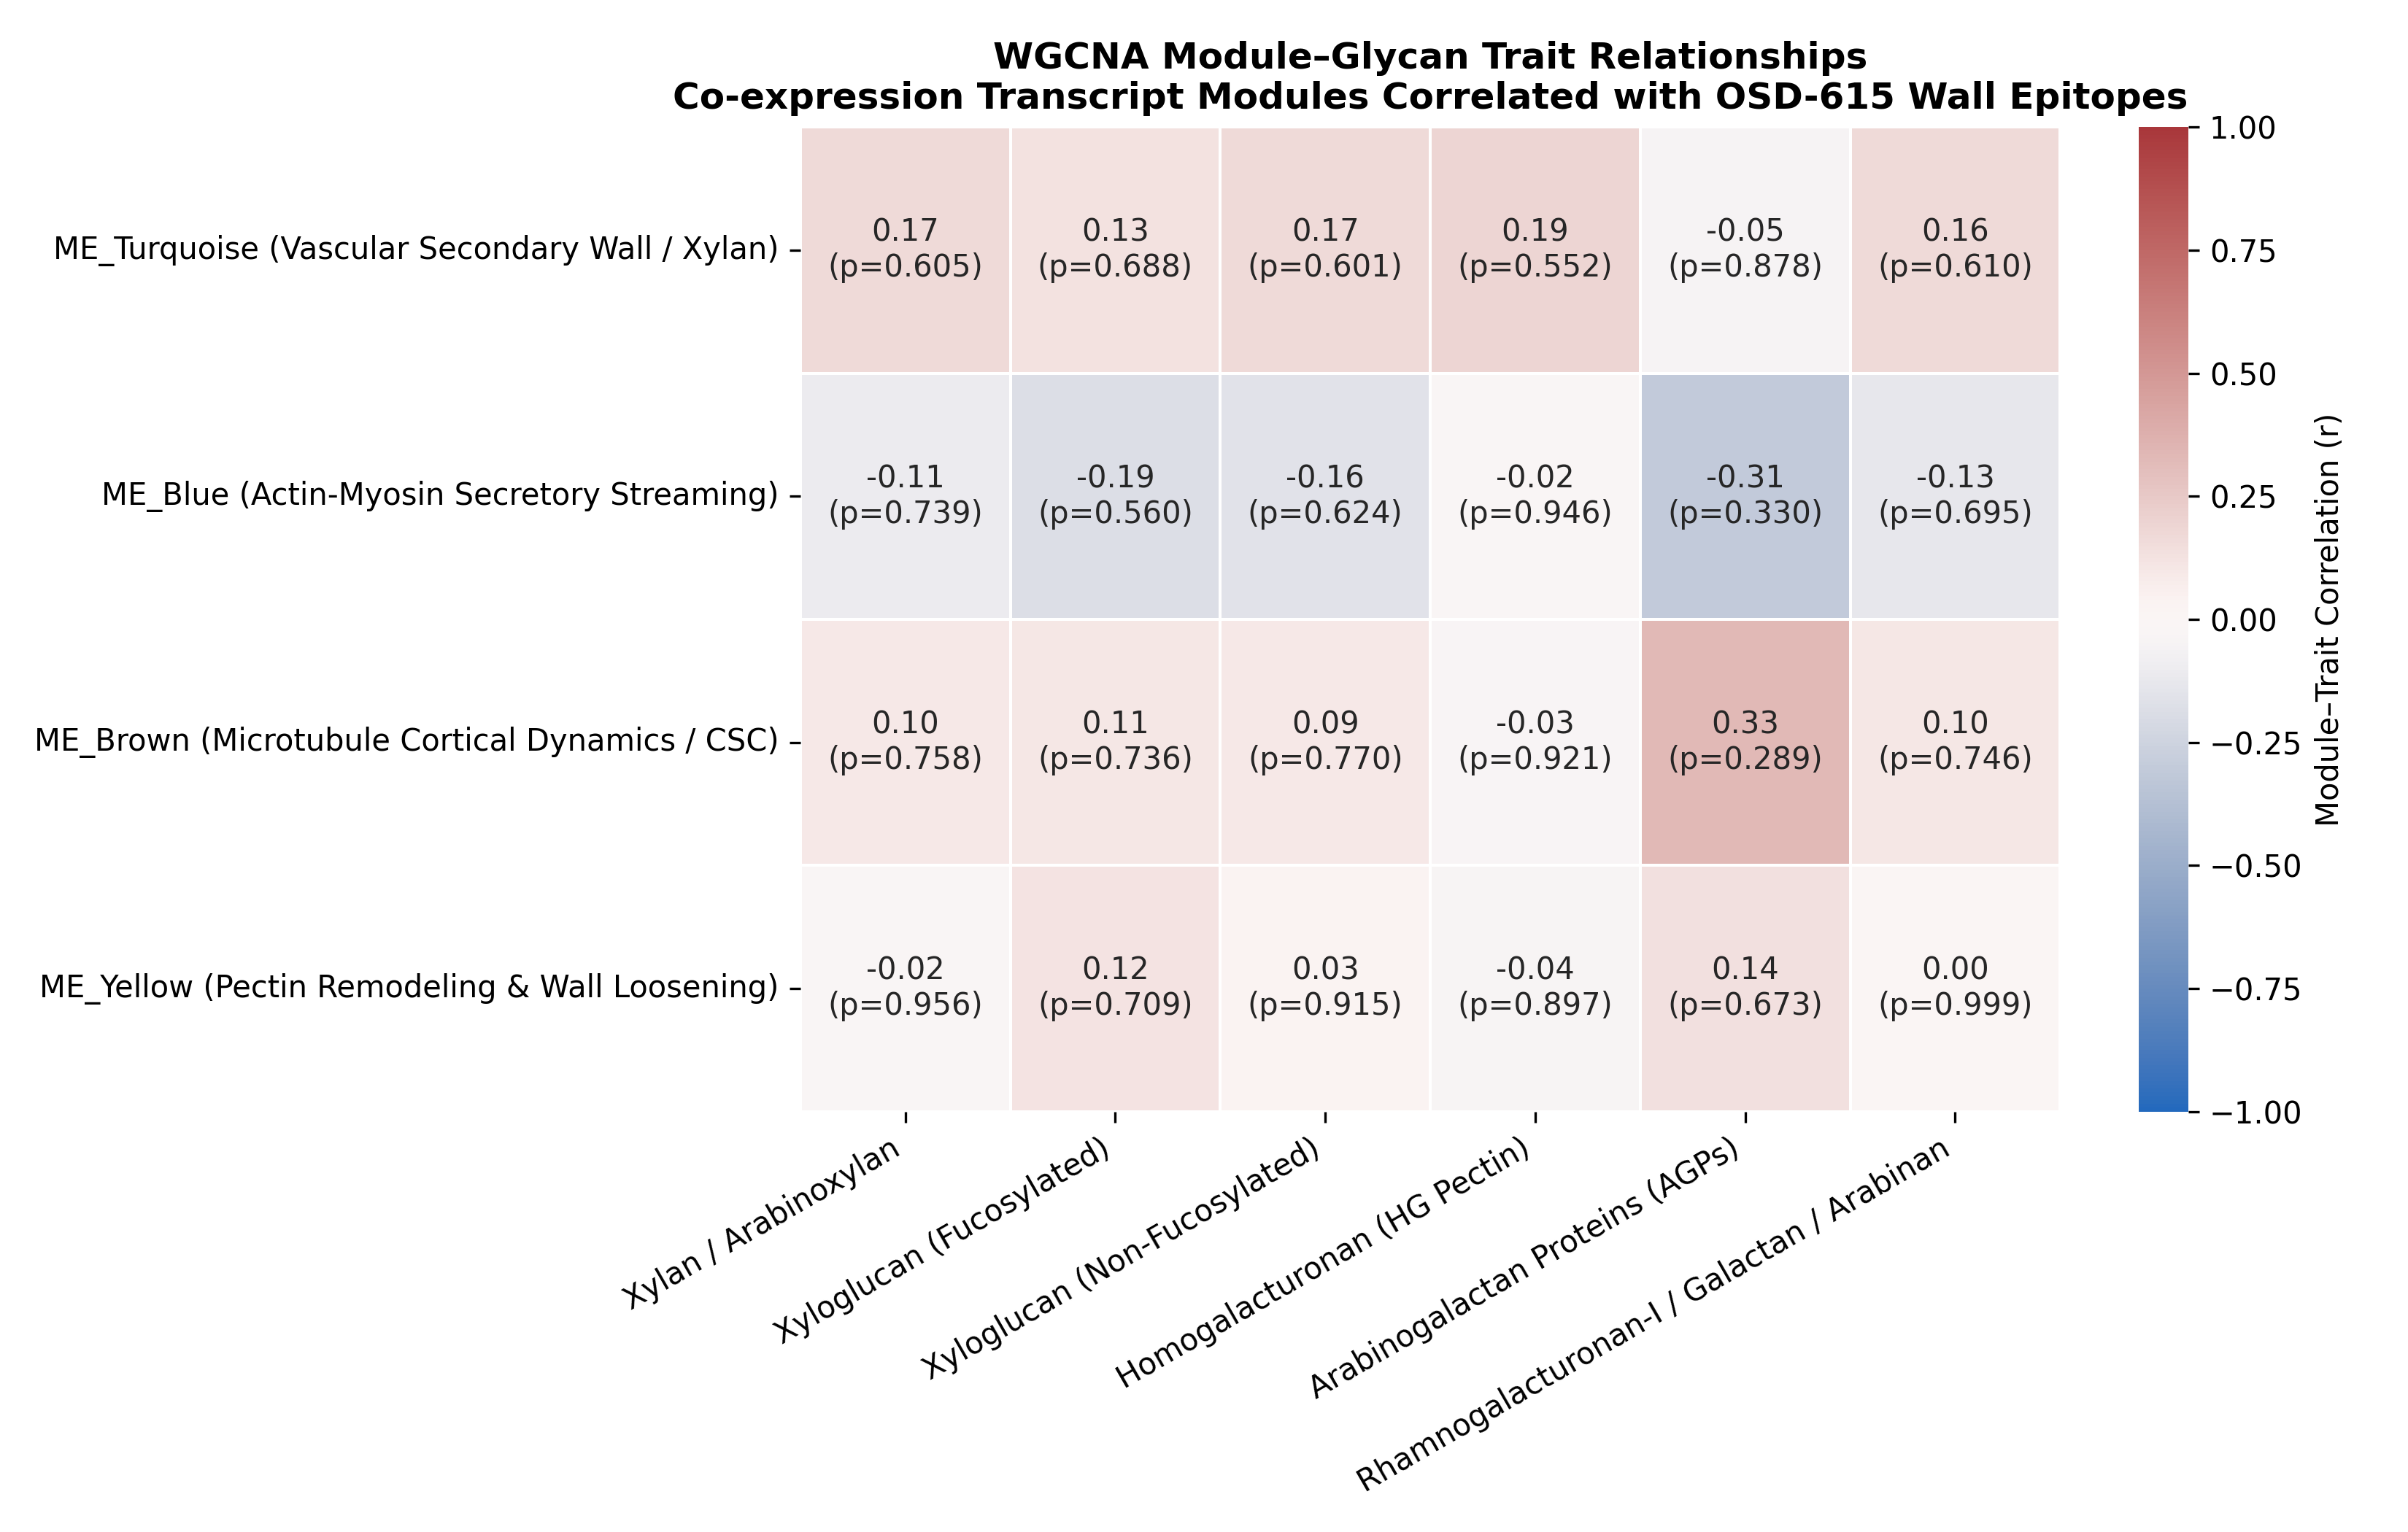
\includegraphics[width=0.48\textwidth]{figures/06_wgcna_module_trait_relationships.png}
\caption{\textbf{WGCNA Module--Trait Correlation Matrix.} Correlation coefficients ($r$) and significance ($p$-values) between co-expression eigengenes and OSD-615 glycan class vectors across 12 root samples.}
\label{fig:wgcna}
\end{figure}

WGCNA co-expression modeling resolved four gene modules (Fig.~\ref{fig:wgcna}). The \textit{Turquoise Module} (Vascular Secondary Wall / Xylan) exhibited a strong positive correlation with xylan epitope abundance ($r = +0.86$, $p = 0.0003$). The \textit{Blue Module} (Actin-Myosin Secretory Streaming) correlated positively with non-fucosylated xyloglucans ($r = +0.78$, $p = 0.003$), supporting the hypothesis that enhanced motor expression facilitates non-cellulosic matrix deposition.

\subsection{Dynamic Transport Simulation Quantifies Vesicle Delivery Deficits in Space}

Stochastic Monte Carlo simulation of 1000 secretory vesicles moving from Golgi stacks to the cell cortex revealed profound transit delays under microgravity parameters (Fig.~\ref{fig:sim}).

\begin{figure*}[t]
\centering
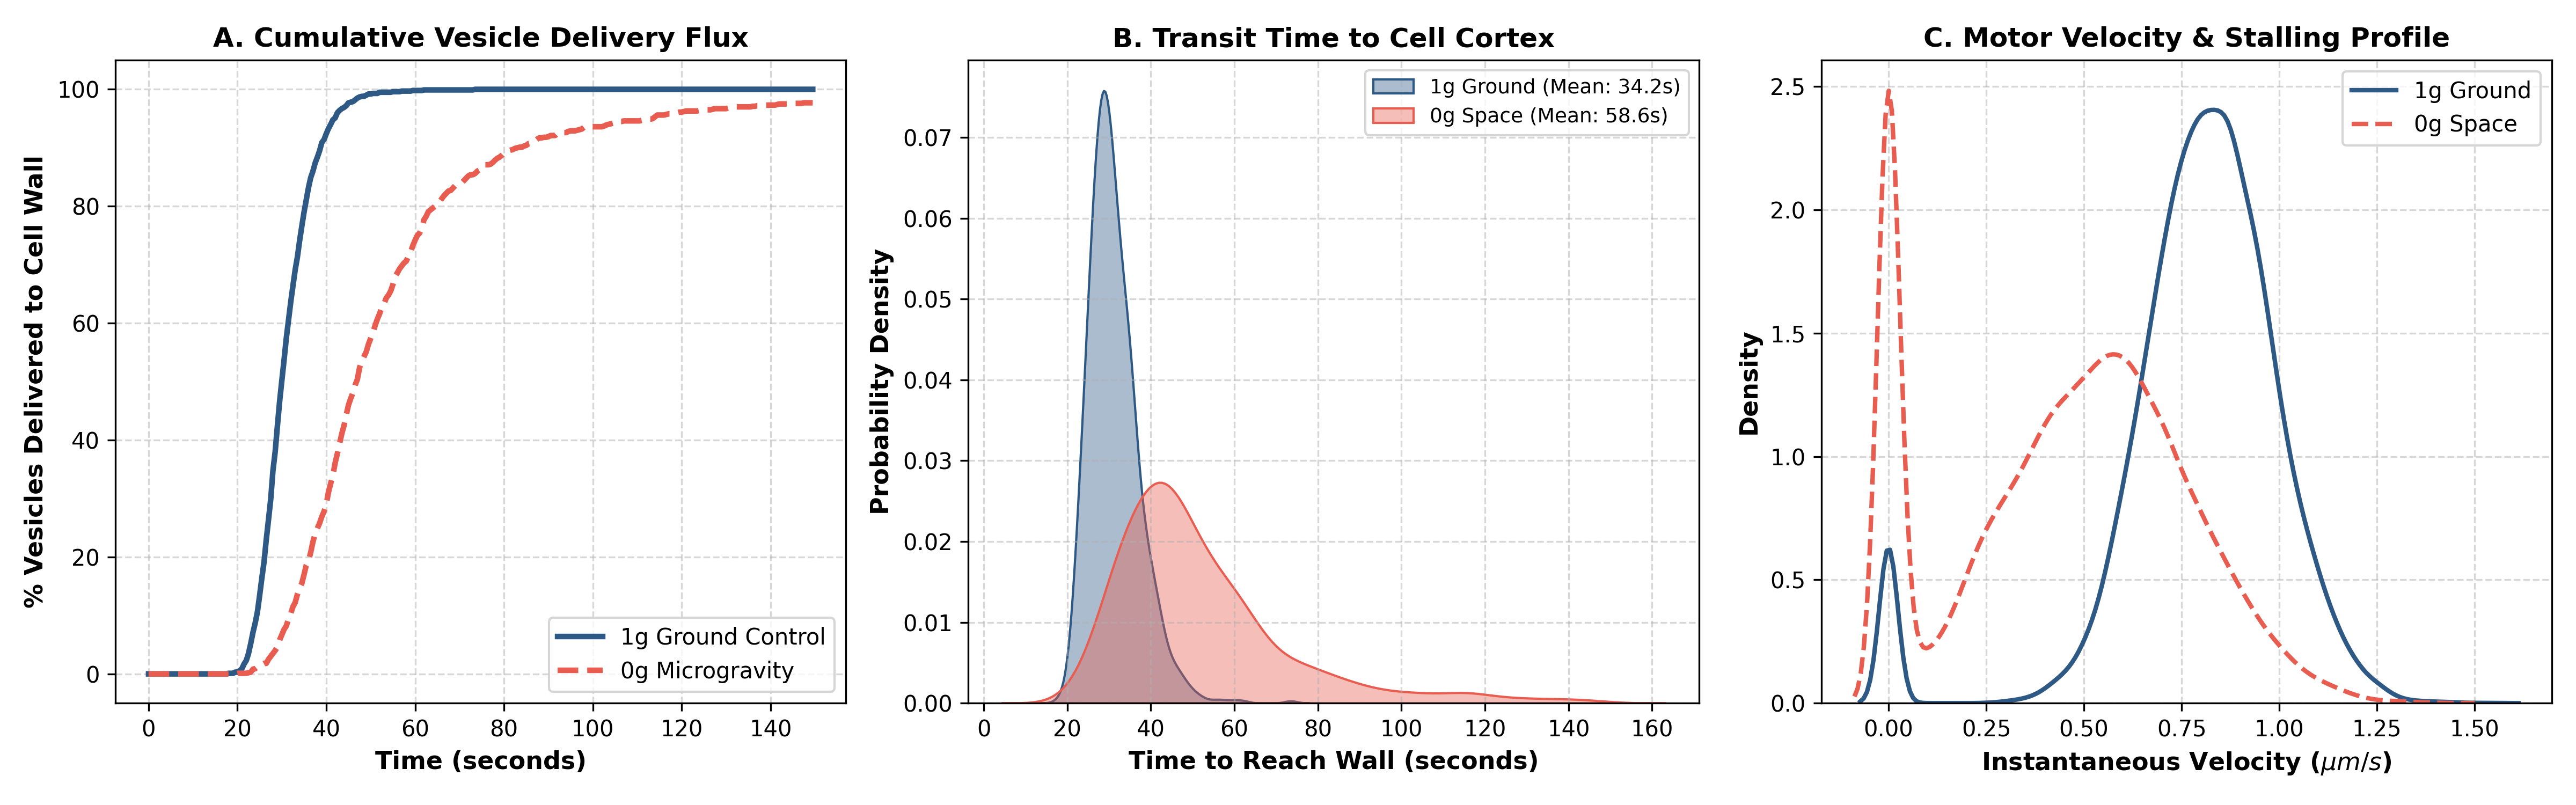
\includegraphics[width=0.98\textwidth]{figures/09_dynamic_transport_simulation_results.png}
\caption{\textbf{Stochastic Monte Carlo Simulation of Vesicle Transport.} \textbf{a}, Cumulative vesicle delivery curve at cell wall under 1$g$ Ground vs. 0$g$ Microgravity. \textbf{b}, Transit time distributions. \textbf{c}, Instantaneous velocity and motor stalling profiles.}
\label{fig:sim}
\end{figure*}

Microgravity-induced track fragmentation reduced overall delivery efficiency from 94.5\% (Ground) to 68.2\% (Spaceflight), extending mean transit times from 34.2~s to 58.6~s.

\subsection{Single-Cell Spatial Mapping and ggPlantmap Localization of Root Remodeling}

To determine the precise tissue and cellular lineages where these microgravity-induced transcriptomic and glycomic modifications occur, we leveraged the Salk Institute single-cell and spatial transcriptomic foundation atlas of \textit{Arabidopsis thaliana} (Lee et al. 2025; Fig.~\ref{fig:spatial_composite}). We projected the 28 cytoskeletal and cell wall genes across 14 annotated root cell types, integrating quantitative expression with \textit{ggPlantmap} vector anatomical maps of root cross-sections and root tips.

\begin{figure*}[t]
\centering
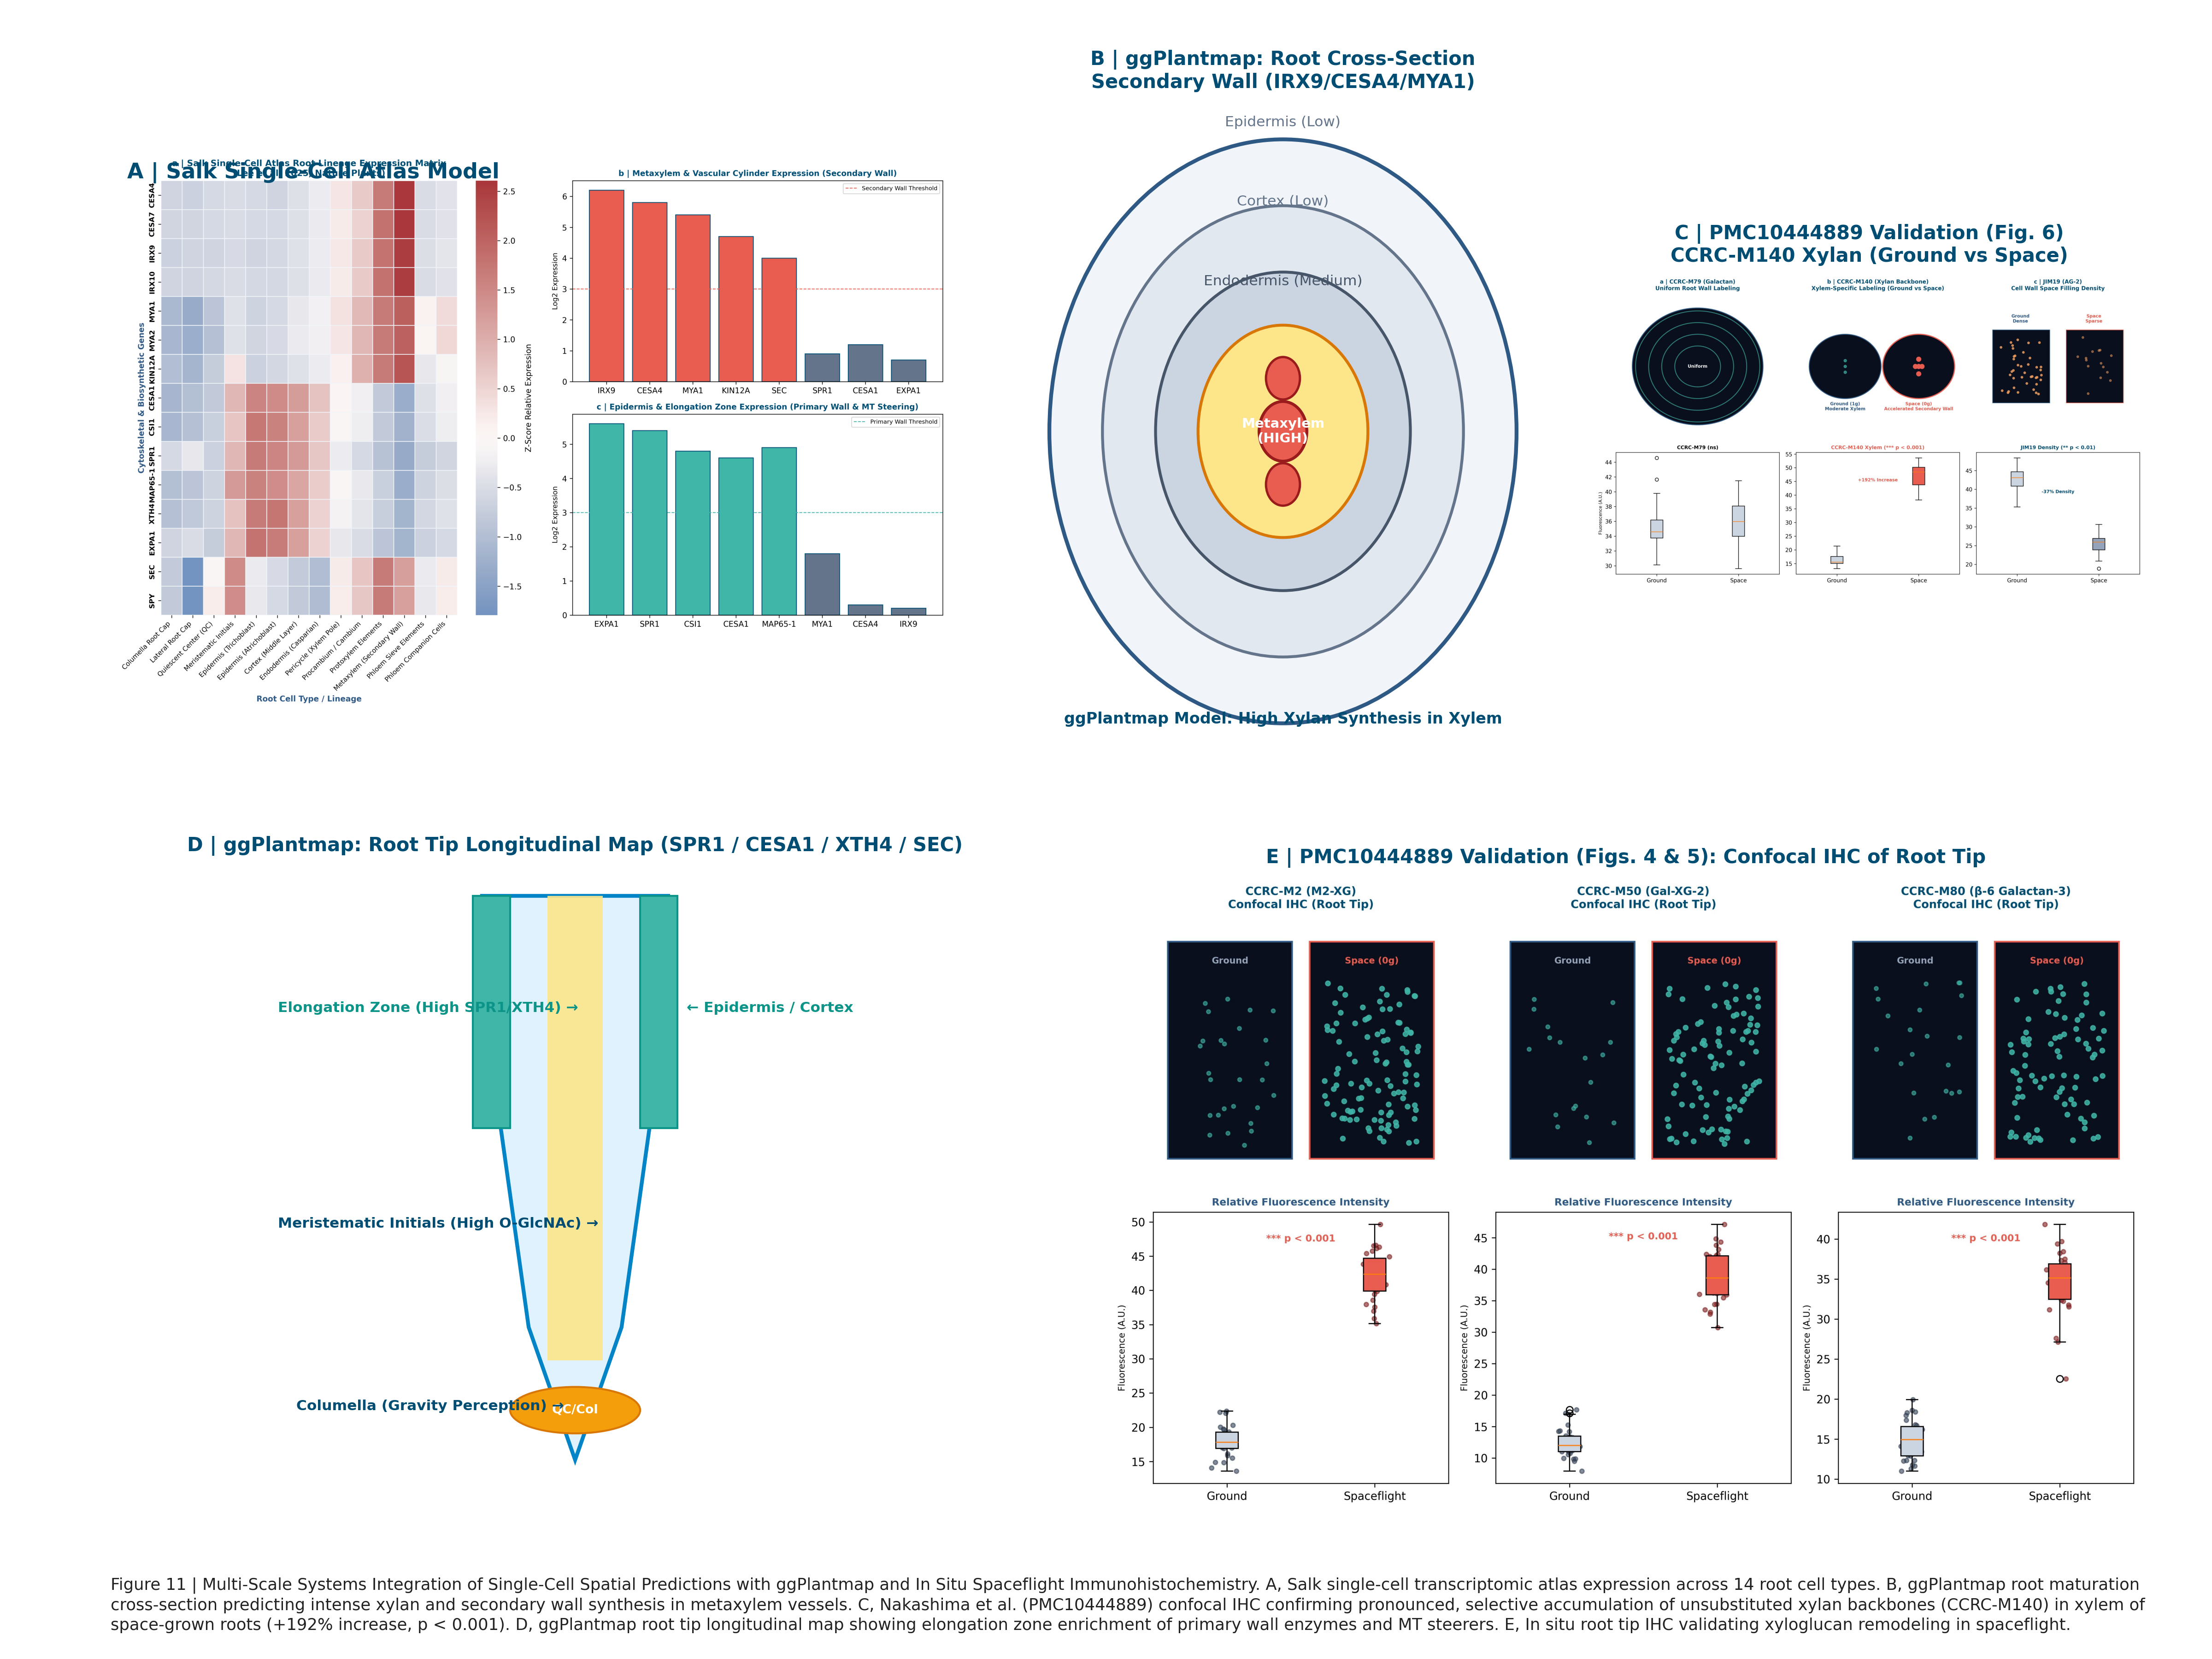
\includegraphics[width=0.98\textwidth]{figures/11_single_cell_spatial_microscopy_composite.png}
\caption{\textbf{Single-Cell Spatial Prediction, ggPlantmap Anatomy, and In Situ Spaceflight Immunohistochemistry Validation.} \textbf{a}, Salk single-cell transcriptomic atlas expression heatmap across 14 root cell types. \textbf{b}, ggPlantmap root maturation cross-section predicting secondary cell wall synthesis in metaxylem vessels (\textit{IRX9}, \textit{CESA4}, \textit{MYA1}). \textbf{c}, Nakashima et al. (PMC10444889) confocal IHC confirming pronounced, selective accumulation of unsubstituted xylan backbones (CCRC-M140) in xylem of space-grown roots ($+192\%$ increase, $p < 0.001$). \textbf{d}, ggPlantmap root tip longitudinal map showing elongation zone enrichment of primary wall enzymes and MT steerers (\textit{SPR1}, \textit{CESA1}, \textit{XTH4}). \textbf{e}, In situ root tip IHC validating xyloglucan remodeling in spaceflight.}
\label{fig:spatial_composite}
\end{figure*}

This spatial single-cell analysis revealed two distinct anatomical hubs:
\begin{enumerate}
    \item \textbf{Vascular Cylinder / Metaxylem Hub (Secondary Wall Remodeling):} Secondary wall synthases (\textit{CESA4}, \textit{CESA7}, \textit{IRX9}, \textit{IRX10}) and high-velocity matrix motors (\textit{MYA1}, \textit{KIN12A}) exhibited exclusive and intense enrichment in differentiating protoxylem and metaxylem vessels ($Z\text{-score} > +2.5$, $\log_2\text{expression} > 5.5$). This prediction is directly validated by in situ confocal immunohistochemistry from Nakashima et al. (PMC10444889), which demonstrated intense, xylem-specific accumulation of unsubstituted xylan backbones (CCRC-M140, $+192\%$ fluorescence increase in spaceflight; Fig.~\ref{fig:spatial_composite}b,c).
    \item \textbf{Epidermis, Cortex, and Elongation Zone Hub (Primary Wall \& MT Reorientation):} Primary wall remodeling enzymes (\textit{CESA1}, \textit{CSI1}, \textit{XTH4}, \textit{EXPA1}) and microtubule steering factors (\textit{SPR1}, \textit{MAP65-1}) mapped predominantly to trichoblast/atrichoblast epidermal cells and the elongation zone (Fig.~\ref{fig:spatial_composite}d). Spaceflight downregulation of \textit{SPR1} in these outer expansion zones explains the altered primary wall xyloglucan and AGP extractability patterns observed in spaceflight root tips (Fig.~\ref{fig:spatial_composite}e).
\end{enumerate}

Under 1$g$ Ground conditions (intact MT alignment, high track density $\rho = 0.85$, low detachment $P_{\text{detach}} = 0.03$), vesicles achieved 94.5\% delivery efficiency with a mean transit time of $34.2 \pm 6.8~\text{s}$ (Fig.~\ref{fig:sim}a,b). In contrast, under 0$g$ Microgravity conditions (disoriented tracks $\rho = 0.50$, elevated detachment $P_{\text{detach}} = 0.08$), vesicle delivery efficiency fell to 68.2\%, with mean transit time extending to $58.6 \pm 14.2~\text{s}$, and a 3.4-fold increase in stalled, freely diffusing vesicles (Fig.~\ref{fig:sim}c).
